\chapter{Background}
\label{chapter:background}

\section{A Brief Introduction to Reservoir Computing}
\label{section:reservoir-computing-introduction}

Recurrent Neural Networks (RNNs), as opposed to feed-forward neural networks,
are notoriously time consuming and difficult to train \cite{Schrauwen2007}.
This is due to feedback from the recurrent connections during the training process,
allowing small topology changes to drastically change a network's position in the fitness landscape.

It was therefore proposed in both \cite{jaeger2002adaptive} as Echo State Networks (ESNs)
and \cite{natschlager2002liquid} as Liquid State Machines (LSMs) to separate the RNN into two parts,
the untrained recurrent reservoir, and the trained readout layer.
The LSM and ESN methods have been unified into the field of Reservoir Computing,
now focusing on the separate training and evolution of the recurrent and readout parts \cite{lukovsevivcius2012reservoir}.
Exiting applications of Reservoir Computing include speech and handwriting recognition,
as well as controlling robotics \cite{lukovsevivcius2012reservoir}.

\begin{figure}[ht]
    \caption[Schematic of a general reservoir computing system]{
        Schematic of a general Reservoir Computing system containing adjustable biases, feedback loops, reservoir and readout layers,
        which are described in section \ref{section:reservoir-computing-introduction}.
        Inspired by figures from \cite{Schrauwen2007} and \cite{Jaeger:2007}.
    }
    \label{fig:rc-schema}
    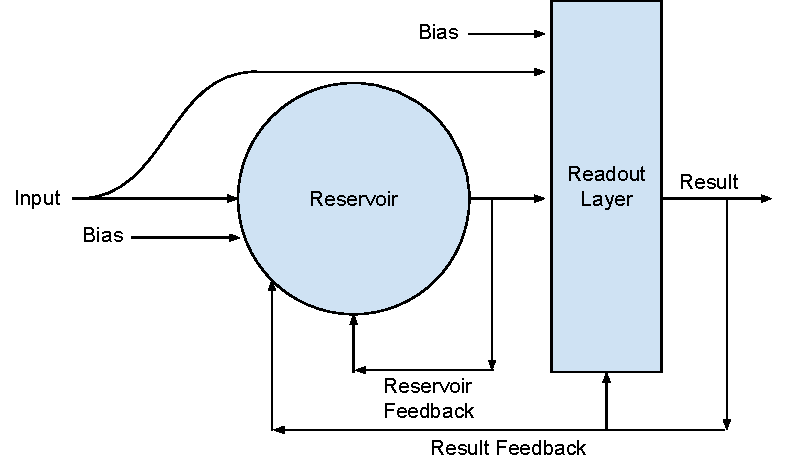
\includegraphics[width=\columnwidth]{background/reservoir_computing_schema.pdf}
\end{figure}

A generalized model of a Reservoir Computing system is shown in figure \ref{fig:rc-schema}.
The main components are the reservoir and the readout layer.
At each time step in the core model,
the reservoir receives the current input signal as well as its previous state.
The reservoir transforms the input, and passes it on to the readout layer.
The readout layer frequently receives the input signal as well.
The internal weights of the reservoir are usually randomized and left untrained,
with the weights of the readout layer being adjusted by some learning algorithm.
This can be linear or ridge regression for offline learning,
or recursive least squares for online learning \cite{Schrauwen2007}.

There are many extensions to the base model.
The reservoir and readout layers can receive a constant bias:
The readout's bias is used for regularizing the reservoir state in case the problem is ill-posed.
This isn't needed when using a model like ridge regression, which performs regularization internally \cite{Schrauwen2007}.
The reservoir's bias is used for stabilizing models which feeds the readout layer back into the reservoir,
which may be needed if the problem entails producing oscillating output \cite{Jaeger:2007}.
Teacher forcing,
that is forcing the states of the readout layer to those expected by the trainer for the first n time steps,
usually speed up the convergence of the learning method used,
and may in some cases be required to at all achieve stability \cite{jaeger2002tutorial}.

For a deeper dive into Reservoir Computing,
consult papers \cite{Schrauwen2007}, \cite{lukovsevivcius2012reservoir}, and \cite{Jaeger:2007}.

\section{Alternatives to Traditional Reservoirs}

Any complex dynamical system can in principle be used in a reservoir computing setting.
What properties must these reservoirs have to be able to solve problems?

Complex networks similar to the sparsely connected ones used in ESN and LSM systems include cellular automata \cite{wolfram2002new} and random Boolean networks \cite{kauffman1969metabolic}.
Cellular automata are regular grids of cells containing some state,
each cell connected to its neighbors in the grid.
Cells then update in lockstep according to some shared transition table,
creating a new generation.
RBNs can be seen upon as an abstraction over CAs again,
allowing for nonlocal neighbors and variable updating rules.
This computational paradigm is known as Cellular Computing,
and provides a potentially powerful alternative to classical computers,
leveraging extreme parallelism, simple components and local state \cite{sipper1999emergence}.

Both CAs and RBNs have successfully been used in reservoir computing systems \cite{yilmaz2014reservoir} \cite{rbn-reservoir}.
The RBN reservoir computing approach will be referred to as RBN RC.
Both models are simple, and can be implemented in software,
hardware such as FPGAs, and in materio \cite{miller2002evolution} \cite{farstad2015evolving}.

\section{A Brief Introduction to Boolean Networks}
\label{section:rbns}

Random Boolean networks were originally developed as a model of gene regulatory networks \cite{kauffman1969metabolic},
the complex system that regulates how genes in multicellular organisms interact with each other.
The model requires no assumptions about the inner workings of the actual nodes,
which allows it to model phenomena where the exact internal workings of the system may be unknown.

The simplification of a system to a Boolean model doesn't pose a problem,
as any multivalued network can be transformed to a corresponding binary one.

A RBN is usually described by its number of nodes $N$ and the in-degree $K$ of the nodes,
that is, how many nodes each node depends on (also known as its ancestors).
RBNs can have both homogeneous and heterogeneous in-degrees.
In heterogeneous networks, one usually describes the average connectivity $\langle K \rangle$ instead.

Each node can have a state of zero or one.
The next state of the node is solely determined by the current combination of states of its ancestors.
Each combination leads to a new state of zero or one,
with the probability given by a binomial distribution usually having $\langle P \rangle = 0.5$.
Figure \ref{figure:sample-homogenous-rbn} visualizes a homogeneous RBN with $N=3, K=2, P=0.5$.

\begin{figure}
  \centering
  \subfloat[RBN topology]{
    \begin{tikzpicture}[node distance = 5em]
      \node[vertex] (a) {a};
      \node[vertex] (b) [below left of=a] {b};
      \node[vertex] (c) [below right of=a] {c};

      \draw[edge] (a) to[bend right] (b);
      \draw[edge] (a) to (c);

      \draw[edge] (b) to (a);
      \draw[edge] (b) to[bend right] (c);

      \draw[edge] (c) to[bend right] (a);
      \draw[edge] (c) to (b);
    \end{tikzpicture}
  }
  \subfloat[Transition table for node a]{
    \begin{tabular}[b]{ c c | c}
      \multicolumn{2}{c}{Ancestor states} & New state \\
      \hline
      0 & 0 & 0 \\
      0 & 1 & 1 \\
      1 & 0 & 0 \\
      1 & 1 & 1 \\
    \end{tabular}
  }
  \caption[An example homogeneous RBN]{An example homogeneous RBN with $N=3, K=2, P=0.5$.}
  \label{figure:sample-homogenous-rbn}
\end{figure}

In the simplest RBN updating scheme, all nodes update in lockstep.
This is known as the Classical RBN updating scheme (CRBN).
The states of the RBN at the next time step $t+1$ therefore only depend on the states at the previous time step $t$.
As the number of RBN states is finite ($2^{n\_nodes}$),
the system will eventually revisit a previously visited state.
This set of repeating states is known as an \emph{attractor},
and a deterministic system cannot escape from it.
If the attractor consists of a single state it is known as a point attractor,
otherwise a cycle attractor.
The set of states leading towards an attractor is known as its \emph{basin of attraction}.
A cycle attractor can be observed in figure \ref{figure:rbn-critical},
while a point attractor is observed in figure \ref{figure:rbn-ordered}.

A criticism of the classical model is that gene regulation networks are updating continuously,
as opposed to in lockstep \cite{gershenson2004introduction}.
There are therefore a number of alternate updating schemes which can be categorized by whether they are deterministic or nondeterministic, as well as synchronous and asynchronous.

The dynamics of a RBN can be categorized as being in either the ordered, critical, or chaotic phase.
These phases can be identified by how large a part of the network state is able to change over time,
whether similar states tend to converge or diverge over time,
and the networks resistance to perturbations (outside changes to the network).

One way to obtain these phases analytically is by comparing the resulting states of two identical RBNs where one is subject to some perturbation \cite{gershenson2004introduction}.
For visual identification, we plot the states of the RBN in a square lattice,
with the network states plotted horizontally, and time flowing downwards.
A node is drawn as white if its state is one, black otherwise.
The phases are visualized in figure \ref{figure:rbn-phases}.

\begin{figure}
  \subfloat[Ordered phase, K=1]{
    
\includegraphics[width=0.3\columnwidth]{background/ordered-phase.pdf}
    \label{figure:rbn-ordered}
  }
  \subfloat[Critical phase, K=2]{
    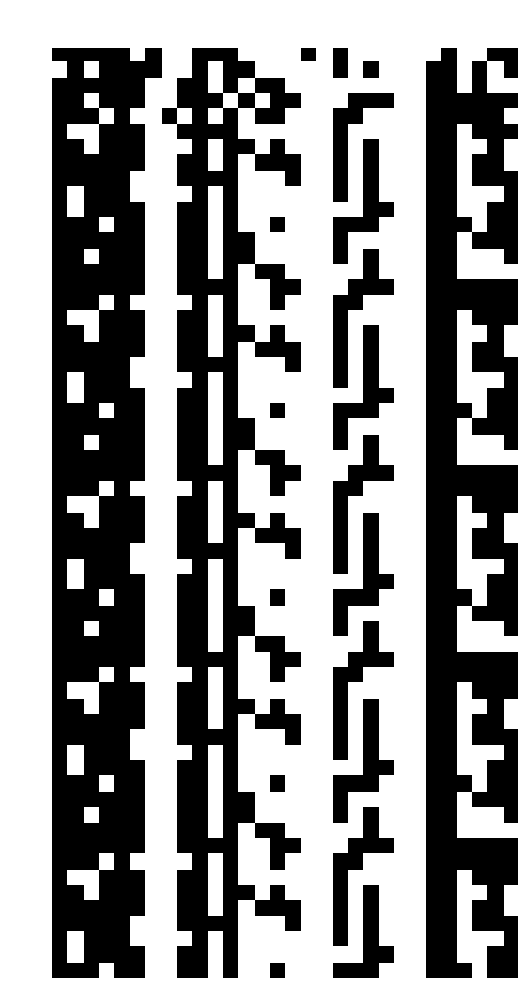
\includegraphics[width=0.3\columnwidth]{background/critical-phase.pdf}
    \label{figure:rbn-critical}
  }
  \subfloat[Chaotic phase, K=3]{
    
\includegraphics[width=0.3\columnwidth]{background/chaotic-phase.pdf}
    \label{figure:rbn-chaotic}
  }
  \caption[Trajectories through state space for RBNs with different connectivities] {
    Trajectories through state-space for RBNs with $N=30, K=[1,2,3]$, visualizing the different phases.
    Time flows downwards the lattice, while RBN states are shown along the X-axis.
    with the network states plotted horizontally, and time flowing downwards.
    Images created with the developed RBN-simulator.
  }
  \label{figure:rbn-phases}
\end{figure}

In general, RBNs in the critical phase are the most interesting.
These are seemingly able to support information transmission, storage and modification,
all capacities required for computation \cite{langton3computation}.
Critical systems are found on the edge of chaos,
on the phase transition between ordered and chaotic networks \cite{gershenson2004introduction}.
For RBNs with $\langle p \rangle = 0.5$,
critical dynamics are usually found at $\langle K \rangle = 2$ \cite{gershenson2004introduction},
although one could still find networks with such dynamics for different values of $\langle K \rangle$.

A thorough introduction to the field of RBNs is available in \cite{gershenson2004introduction}.

\section{RBN Reservoir Computing systems}
\label{subsection:rbn-reservoir-systems}

How does one adapt a RBN for use as a reservoir in a RBN RC device?
RBNs aren't usually designed to take external input.
We do however, have the concept of perturbation,
the external flipping of bits in the network's state,
transition tables or edges.
This can be utilized to create RBNs that take input,
by continuously perturbing the RBN nodes by the bits of the input sequence.

Questions that follow are how many bits should the network consume at a time,
how many of the network nodes should be perturbed by the input at each time step,
and what dynamics must such a reservoir have to allow for the computation of interesting problems?

\subsection{A working system}

In \cite{rbn-reservoir} functioning RBN RC systems are created and analyzed.
These RBN RC systems have heterogeneous connectivity,
consume one bit of input at each time step ($I=1$),
perturbing $IC$ of the $N$ nodes in the process.
The readout layer can be any node performing some kind of regression of the reservoir state against expected output for the current task, e.g. linear regression.
Such a setup is shown in figure \ref{figure:rbn-reservoir}.

\begin{figure}
  \centering
  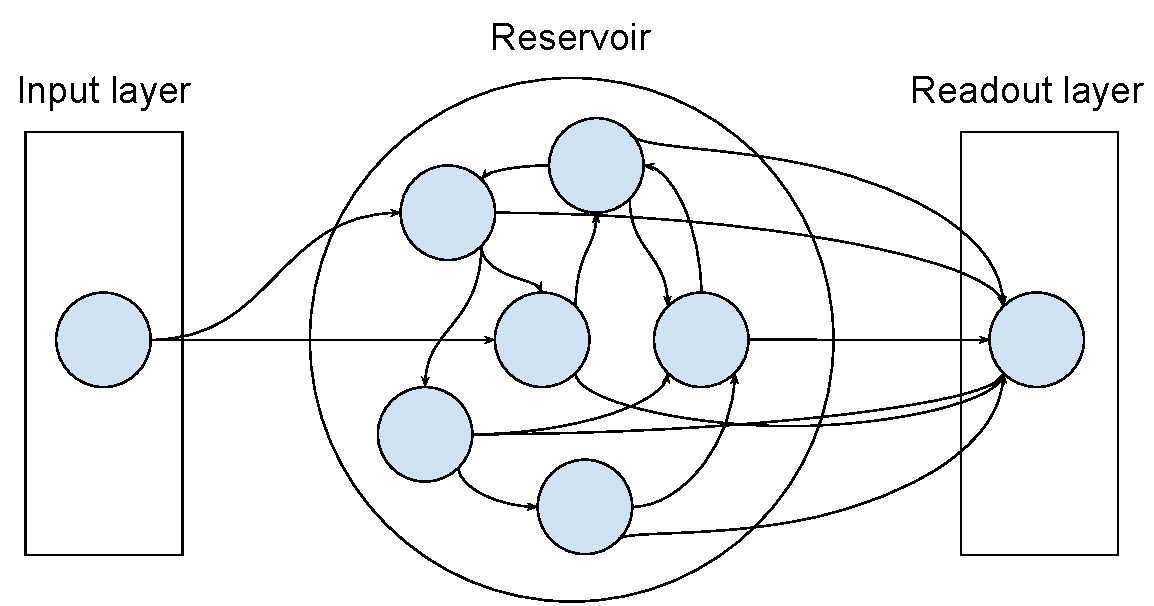
\includegraphics[width=\columnwidth]{background/RBN-Reservoir.pdf}
    \caption[An example RBN RC system]{
    An example RBN RC system with $I=1, IC=2, K=2, N=6$ with the entire reservoir sate used for regression.
    The reservoir transforms the problem from a temporal one to a multidimensional spatial one.
    The readout layer the performs some kind of learning on the reservoir states against the expected output for the current task.}
  \label{figure:rbn-reservoir}
\end{figure}

\subsection{Tasks}
\label{section:tasks}

To measure the real-life performance and accuracy of the RBN RC system,
two tasks are introduced: Temporal density and temporal parity \cite{rbn-reservoir}.
Both require the reservoir to be able to retain information for a sliding window of size $ n $,
offset by some value $ t $, back through the input stream.
The temporal parity task requires us to determine if there were an odd number of ones in the sliding window,
the temporal density task to determine whether there were a majority of ones.
The Former is visualized in figure \ref{figure:temporal-parity}.

Both tasks will be used to benchmark the reservoirs created later in this paper.

\begin{figure}
  \subfloat[Input]{
    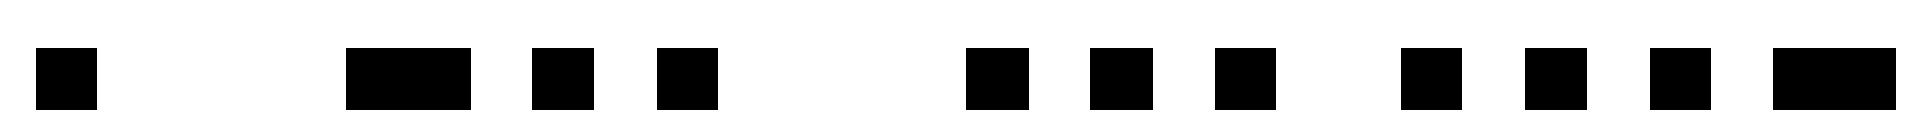
\includegraphics[width=\columnwidth]{background/temporal_parity-10-200-3-input.pdf}
  }

  \subfloat[Correct output]{
    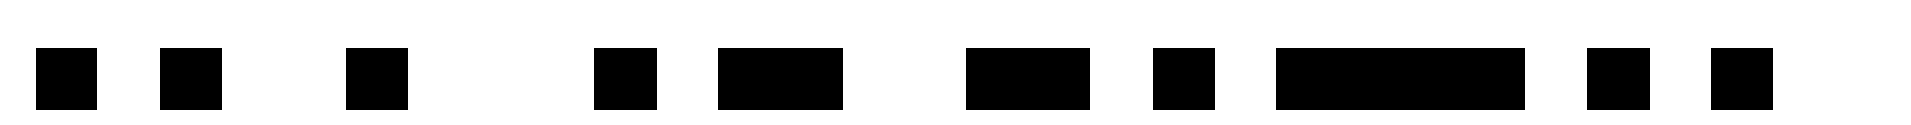
\includegraphics[width=\columnwidth]{background/temporal_parity-10-200-3-output.pdf}
  }

  \caption[The first elements of the temporal parity task]{
    The first 30 elements of a temporal parity task with $[n=3, t=0]$.
    A one is visualized as white, while a zero is black.
    We see that correct output at time $i$ is equal to there being an odd number of $1$s in inputs $[i, i-1, i-2]$
  }
  \label{figure:temporal-parity}
\end{figure}

\subsection{Computational capability}
\label{section:computational-capability}
For a RBN-reservoir to perform well at computational tasks,
it must be able to both forget past perturbations and keep two input streams that have begun converging separated \cite{bertschinger2004real}.

These two properties are coined \textit{fading memory} and \textit{separation property},
and can be measured \cite{rbn-reservoir} as follows.

Create two equal input streams \#1 and \#2 of length $T$.
If measuring \textit{fading memory}, flip the first bit in stream \#2.
If measuring \textit{separation property}, flip all bits up to bit $T-t$ in stream \#2
($t$ being the required depth of separation).
For both input streams, reset reservoir state, perturb the reservoir with the input stream,
and store the final state.
The score of the measure is then defined as the normalized hamming distance between the resulting states.
The computational capability $\Delta$ of a RBN-reservoir is then defined as
\begin{equation}
  \Delta_{Tt} = separation\_property_{Tt} - fading\_memory_{T}
\label{formula:accuracy}
\end{equation}
Analyzing different RBN-reservoirs with this metric \cite{rbn-reservoir},
a high $\Delta$ is found to correlate with critical connectivity ($\langle K \rangle = 2$).
For all RBN-reservoirs, $\Delta$ drops when increasing the required separation $t$,
and is maximized when one doesn't have to remember anything at all ($t=0$).

\subsection{Optimal perturbation}
\label{section:optimal-perturbance}
It is found that the optimal amount of reservoir perturbation,
adjustable by the number of connections between the input layer and the reservoir,
depends on both the task size, how many steps in time are required to be remembered,
and the dynamics of the reservoir.
\textit{Chaotic reservoirs} require few input connections to be able to properly spread information,
but perform poorly on larger tasks due to past perturbations still floating around the reservoir.
\textit{Ordered reservoirs} quickly forget past perturbations, allowing some success for larger tasks,
but their inability to remember past perturbations renders them useless for many tasks.
\textit{Critical reservoirs} require connectivity somewhere in the middle.
Able to forget as well as remember, they perform accurately independent of task size.


\section{Evolution in Materio and physical reservoirs}
\label{section:evo-materio-physical-reservoirs}

The field of evolution-in-materio \cite{miller2002evolution} concerns the harnessing of unconventional and complex physical materials,
using them to perform computation.
The process is usually aided by Artificial Evolution for finding reasonable input-substrate-output mappings.
The difference from classical computation is that the computation is moved from an abstraction over the hardware (e.g. a modern CPU), and into the material itself.
This material can be anything from grown dendritic iron wires which discriminate sound \cite{pask1958physical} to carbon nanotubes used for evolving CA rules \cite{farstad2015evolving}.
Success within this field may result in more efficient use of materials,
and higher computational densities.

In \cite{demarse2005adaptive},
living rat neurons are put in a microelectrode array (MEA) and successfully used to control an airplane in a flight simulator.
Two of sixty electrodes were chosen to control the pitch and roll of the airplane.
The internal 'weights' of the rat brain were trained by administering a series of electrical impulses to the same electrodes which then increase or decrease the action potential of the region,
correcting behavior.
The internal state of the system is unknown,
with the MEA only exposing a limited resolution subset of the entire system state
(around 60 electrodes).

In \cite{farstad2015evolving}, the computational power of carbon nanotubes,
instrumented in a microelectrode array,
is used to evolve the state transition functions of all elementary Cellular Automata.
Artificial Evolution is used to find the correct translation of input/output values to their respective electrodes.
The internal state of the carbon nanotubes are again completely opaque to the higher computational layers.
In addition, the number of electrodes present a limited resolution view of the substrate.

In the ever-so-cited 'Pattern recognition in a bucket' paper \cite{fernando2003pattern},
the Liquid State Machine metaphor is taken literally and a bucket of water is used as a physical reservoir.
The bucket of water receives input via rotors mounted on the edge of the bucket.
Input is then transformed from a temporal into a spatial, with a great deal of nonlinearity introduced by the bucket.
Finally, the reservoir state is read out by taking pictures of the wave-patterns,
using a simple perceptron to classify the resulting state.
This setup correctly separates the xor problem as well as being able to classify the words 'one' and 'zero' when yelled into the bucket.

What these approaches have in common is that physical substrates,
with varying degrees of perturbation ability and insight into the internal state,
are used for computation.
Their couplings to theoretical frameworks such as Reservoir Computing motivate the exploration of the effects of limited perturbation and readout possibilities on reservoir performance.

\section{Validating RBNs for Reservoir Computing}
\label{section:pre-thesis-project}

In the authors pre-thesis paper, the dynamics, performance, and viability of RBN RC systems was investigated.
A functioning RBN RC system was implemented,
and its results validated against and found in accordance with those from \cite{rbn-reservoir}.
The simulation software from the pre-thesis work has been greatly extended for use in this thesis.

A positive correlation between the computational capability (section \ref{section:computational-capability}) of a reservoir and its actual performance is found.
The optimal connectivity for homogeneous reservoirs is found to be $K=3$ as opposed to $\langle K \rangle = 2$ for heterogeneous reservoirs \cite{rbn-reservoir}.
Finally, the required input connectivity is found to rise with the presence of chaotic dynamics in the reservoir.
The figures backing this conclusion are shown in \ref{figure:results:temporal-parity-3} and \ref{figure:results:temporal-parity-5}.

Finally, a one-to-many mapping between the readout layer of an already-trained RBN RC system and different RBN RC is found,
with there being a seemingly large set of interchangeable reservoirs for each readout layer.
This neutrality in the space of possible RBNs make the potential use of a smaller generative genome for evolving RBN RC systems interesting.
Even though such a genome will hit fewer points in the RBN fitness landscape than a fixed genome,
a large amount of these points will still be usable for each instance of a working readout layer.
There doesn't seem to be a tight correlation between the properties of the RBN from the original RBN RC system,
and the equivalent RBNs found through artificial evolution.
In fact, the connectivity distributions of figure \ref{figure:evolved-connectivity} and the computational capabilities of figure \ref{figure:evolved-ccs} seem much more representative of the general RBN population, as shown in figure \ref{fig:res:d-100-3-2}.
This indicates that while there are many compatible reservoirs for a given readout layer,
the distribution of these compatible reservoirs are likely the same as the distribution of reservoirs with the same connectivity in general.

The parameters for the temporal parity task used for all experiments is shown in table \ref{table:pre-thesis-tasks} of appendix \ref{app:pre-thesis-bonus-content}.

\begin{figure*}[ht]
    \centering
    \caption[Computational capability and input connectivity for evolved RBNs]{
        Computational Capability and Input Connectivity distributions for RBNs evolved from a fixed readout layer.
        The Y-axis shows the CC and IC values for the readout layers original RBN.
    }
    \resizebox{\textwidth}{!}{
        \subfloat[Evolved RBN input connectivity]{
            \begin{tikzpicture}
    \begin{axis}
        [
            xlabel=Computational Capability,
            ytick={1,2,3,4,5},
            yticklabels={
                {0.05},
                {0.06},
                {0.05},
                {0.005},
                {0.00}
            },
            yticklabel style={font=\small},
            x tick label style={/pgf/number format/fixed},
        ]
        \addplot+[boxplot]
        table[y index=0] {background/pre-project/final-1-computational-power.dat};

        \addplot+[boxplot]
        table[y index=0] {background/pre-project/final-2-computational-power.dat};

        \addplot+[boxplot]
        table[y index=0] {background/pre-project/final-3-computational-power.dat};

        \addplot+[boxplot]
        table[y index=0] {background/pre-project/N100K2L70-1-computational-power.dat};

        \addplot+[boxplot]
        table[y index=0] {background/pre-project/N100K2L70-2-computational-power.dat};
    \end{axis}
\end{tikzpicture}

            \label{figure:evolved-ccs}
        }

        \subfloat[Evolved RBN Computational Capability]{
            \begin{tikzpicture}
    \begin{axis}
        [
            xmin=30, xmax=70,
            axis x discontinuity=crunch,
            xlabel=Input Connectivity,
            ytick={1,2,3,4,5},
            yticklabels={
                {50},
                {50},
                {50},
                {70},
                {70}
            },
            yticklabel style={align=center, font=\small},
        ]
        \addplot+[boxplot]
        table[y index=0] {background/pre-project/final-1-connectivity.dat};

        \addplot+[boxplot]
        table[y index=0] {background/pre-project/final-2-connectivity.dat};

        \addplot+[boxplot]
        table[y index=0] {background/pre-project/final-3-connectivity.dat};

        \addplot+[boxplot]
        table[y index=0] {background/pre-project/N100K2L70-1-connectivity.dat};

        \addplot+[boxplot]
        table[y index=0] {background/pre-project/N100K2L70-2-connectivity.dat};
    \end{axis}
\end{tikzpicture}

            \label{figure:evolved-connectivity}
        }
    }
\end{figure*}

\begin{figure*}
    \centering
    \caption[Temporal parity 3: Accuracy and computational capability plots]{
        Plots for temporal parity with $N=3$.
        Figures \ref{fig:res:d-100-3-1}--\ref{fig:res:d-100-3-3} plot the accuracies of the sampled RBNs against their input connectivity,
        for K=1–3 respectively.
        Figures \ref{fig:res:c-100-3-1}--\ref{fig:res:c-100-3-3} plot the accuracy of the previous figures against their Computational Capability ($T=100, t=3$).
    }
    \label{figure:results:temporal-parity-3}
    \resizebox{\textwidth}{!}{
        \subfloat[K=1]{
            \label{fig:res:d-100-3-1}
            \myboxplot{
% L: 0
\addplot[mark=*,boxplot, boxplot/draw position=0]
table[row sep=\\, y index=0] {
data
0.52 \\
0.52 \\
0.48 \\
0.52 \\
0.52 \\
0.48 \\
0.52 \\
0.52 \\
0.52 \\
0.52 \\
0.47 \\
0.52 \\
0.56 \\
0.52 \\
0.47 \\
0.52 \\
0.52 \\
0.52 \\
0.52 \\
0.52 \\
0.47 \\
0.52 \\
0.48 \\
0.47 \\
0.52 \\
0.43 \\
0.52 \\
0.52 \\
0.47 \\
0.52 \\
};
% L: 1
\addplot[mark=*,boxplot, boxplot/draw position=1]
table[row sep=\\, y index=0] {
data
0.55 \\
0.465 \\
0.47 \\
0.36 \\
0.48 \\
0.465 \\
0.47 \\
0.425 \\
0.47 \\
0.455 \\
0.485 \\
0.475 \\
0.48 \\
0.44 \\
0.465 \\
0.645 \\
0.47 \\
0.48 \\
0.36 \\
0.48 \\
0.36 \\
0.48 \\
0.48 \\
0.465 \\
0.52 \\
0.48 \\
0.495 \\
0.48 \\
0.36 \\
0.475 \\
};
% L: 2
\addplot[mark=*,boxplot, boxplot/draw position=2]
table[row sep=\\, y index=0] {
data
0.465 \\
0.465 \\
0.47 \\
0.36 \\
0.36 \\
0.475 \\
0.48 \\
0.49 \\
0.51 \\
0.48 \\
0.475 \\
0.465 \\
0.465 \\
0.47 \\
0.475 \\
0.465 \\
0.475 \\
0.515 \\
0.48 \\
0.475 \\
0.465 \\
0.465 \\
0.475 \\
0.455 \\
0.455 \\
0.48 \\
0.48 \\
0.475 \\
0.47 \\
0.49 \\
};
% L: 3
\addplot[mark=*,boxplot, boxplot/draw position=3]
table[row sep=\\, y index=0] {
data
0.41 \\
0.47 \\
0.405 \\
0.405 \\
0.54 \\
0.475 \\
0.48 \\
0.5 \\
0.5 \\
0.48 \\
0.4 \\
0.45 \\
0.425 \\
0.485 \\
0.465 \\
0.445 \\
0.355 \\
0.465 \\
0.47 \\
0.475 \\
0.595 \\
0.485 \\
0.525 \\
0.61 \\
0.475 \\
0.645 \\
0.36 \\
0.475 \\
0.49 \\
0.465 \\
};
% L: 4
\addplot[mark=*,boxplot, boxplot/draw position=4]
table[row sep=\\, y index=0] {
data
0.465 \\
0.585 \\
0.645 \\
0.405 \\
0.475 \\
0.465 \\
0.485 \\
0.36 \\
0.465 \\
0.48 \\
0.475 \\
0.545 \\
0.465 \\
0.41 \\
0.485 \\
0.475 \\
0.47 \\
0.465 \\
0.595 \\
0.465 \\
0.41 \\
0.47 \\
0.47 \\
0.495 \\
0.485 \\
0.49 \\
0.465 \\
0.475 \\
0.48 \\
0.48 \\
};
% L: 5
\addplot[mark=*,boxplot, boxplot/draw position=5]
table[row sep=\\, y index=0] {
data
0.465 \\
0.465 \\
0.465 \\
0.57 \\
0.36 \\
0.475 \\
0.465 \\
0.475 \\
0.435 \\
0.475 \\
0.53 \\
0.465 \\
0.48 \\
0.355 \\
0.555 \\
0.47 \\
0.475 \\
0.455 \\
0.465 \\
0.475 \\
0.475 \\
0.475 \\
0.475 \\
0.52 \\
0.425 \\
0.585 \\
0.465 \\
0.465 \\
0.405 \\
0.485 \\
};
% L: 6
\addplot[mark=*,boxplot, boxplot/draw position=6]
table[row sep=\\, y index=0] {
data
0.465 \\
0.54 \\
0.54 \\
0.47 \\
0.475 \\
0.435 \\
0.475 \\
0.405 \\
0.355 \\
0.465 \\
0.465 \\
0.465 \\
0.465 \\
0.47 \\
0.41 \\
0.465 \\
0.465 \\
0.465 \\
0.475 \\
0.475 \\
0.465 \\
0.46 \\
0.645 \\
0.465 \\
0.465 \\
0.475 \\
0.475 \\
0.475 \\
0.465 \\
};
% L: 7
\addplot[mark=*,boxplot, boxplot/draw position=7]
table[row sep=\\, y index=0] {
data
0.465 \\
0.465 \\
0.475 \\
0.645 \\
0.475 \\
0.475 \\
0.465 \\
0.465 \\
0.48 \\
0.465 \\
0.475 \\
0.465 \\
0.395 \\
0.465 \\
0.475 \\
0.465 \\
0.645 \\
0.465 \\
0.475 \\
0.47 \\
0.48 \\
0.475 \\
0.47 \\
0.425 \\
0.475 \\
0.465 \\
0.465 \\
0.475 \\
0.47 \\
0.465 \\
};
% L: 8
\addplot[mark=*,boxplot, boxplot/draw position=8]
table[row sep=\\, y index=0] {
data
0.465 \\
0.465 \\
0.465 \\
0.465 \\
0.465 \\
0.475 \\
0.465 \\
0.465 \\
0.465 \\
0.465 \\
0.475 \\
0.465 \\
0.475 \\
0.465 \\
0.465 \\
0.48 \\
0.465 \\
0.465 \\
0.475 \\
0.465 \\
0.47 \\
0.475 \\
0.465 \\
0.475 \\
0.465 \\
0.465 \\
0.465 \\
0.475 \\
0.465 \\
0.475 \\
};
% L: 9
\addplot[mark=*,boxplot, boxplot/draw position=9]
table[row sep=\\, y index=0] {
data
0.475 \\
0.465 \\
0.475 \\
0.36 \\
0.465 \\
0.535 \\
0.465 \\
0.465 \\
0.535 \\
0.475 \\
0.465 \\
0.595 \\
0.475 \\
0.465 \\
0.475 \\
0.475 \\
0.465 \\
0.475 \\
0.475 \\
0.475 \\
0.465 \\
0.465 \\
0.475 \\
0.475 \\
0.475 \\
0.475 \\
0.465 \\
0.535 \\
0.475 \\
0.535 \\
};
% L: 10
\addplot[mark=*,boxplot, boxplot/draw position=10]
table[row sep=\\, y index=0] {
data
0.535 \\
0.535 \\
0.535 \\
0.535 \\
0.535 \\
0.535 \\
0.535 \\
0.535 \\
0.535 \\
0.535 \\
0.535 \\
0.535 \\
0.535 \\
0.535 \\
0.535 \\
0.535 \\
0.535 \\
0.535 \\
0.535 \\
0.535 \\
0.535 \\
0.535 \\
0.535 \\
0.535 \\
0.535 \\
0.535 \\
0.535 \\
0.535 \\
0.535 \\
0.535 \\
};
}{0.1}{Input Connectivity}{10}

        }
        \subfloat[K=1]{
            \label{fig:res:c-100-3-1}
            \myscatterplot{background/pre-project/computational-power-100-3-1.dat}
        }
    }

    \resizebox{\textwidth}{!}{
        \subfloat[K=2]{
            \label{fig:res:d-100-3-2}
            \myboxplot{
% L: 0
\addplot[mark=*, mark=*,boxplot, boxplot/draw position=0]
table[row sep=\\, y index=0] {
data
0.545 \\
0.59 \\
0.465 \\
0.465 \\
0.515 \\
0.515 \\
0.515 \\
0.465 \\
0.515 \\
0.515 \\
0.515 \\
0.465 \\
0.59 \\
0.515 \\
0.525 \\
0.515 \\
0.465 \\
0.515 \\
0.545 \\
0.465 \\
0.515 \\
0.56 \\
0.515 \\
0.525 \\
0.465 \\
0.525 \\
0.565 \\
0.515 \\
0.515 \\
0.515 \\
};
% L: 1
\addplot[mark=*, mark=*,boxplot, boxplot/draw position=1]
table[row sep=\\, y index=0] {
data
0.595 \\
0.605 \\
0.99 \\
0.635 \\
0.99 \\
0.57 \\
0.525 \\
0.605 \\
0.99 \\
0.515 \\
0.58 \\
0.58 \\
0.57 \\
0.58 \\
0.755 \\
0.57 \\
0.605 \\
0.535 \\
0.585 \\
0.545 \\
0.565 \\
0.62 \\
0.6 \\
0.585 \\
0.57 \\
0.62 \\
0.515 \\
0.58 \\
0.885 \\
0.57 \\
};
% L: 2
\addplot[mark=*, mark=*,boxplot, boxplot/draw position=2]
table[row sep=\\, y index=0] {
data
0.55 \\
0.555 \\
0.99 \\
0.585 \\
0.84 \\
0.54 \\
0.6 \\
0.99 \\
0.535 \\
0.99 \\
0.935 \\
0.56 \\
0.825 \\
0.555 \\
0.59 \\
0.535 \\
0.55 \\
0.565 \\
0.815 \\
0.99 \\
0.545 \\
0.99 \\
0.56 \\
0.625 \\
0.83 \\
0.99 \\
0.58 \\
0.935 \\
0.57 \\
0.53 \\
};
% L: 3
\addplot[mark=*, mark=*,boxplot, boxplot/draw position=3]
table[row sep=\\, y index=0] {
data
0.99 \\
0.99 \\
0.935 \\
0.61 \\
0.99 \\
0.99 \\
0.99 \\
0.97 \\
0.99 \\
0.71 \\
0.72 \\
0.635 \\
0.625 \\
0.99 \\
0.905 \\
0.57 \\
0.845 \\
0.73 \\
0.99 \\
0.99 \\
0.99 \\
0.89 \\
0.99 \\
0.97 \\
0.855 \\
0.99 \\
0.975 \\
0.99 \\
0.99 \\
0.99 \\
};
% L: 4
\addplot[mark=*, mark=*,boxplot, boxplot/draw position=4]
table[row sep=\\, y index=0] {
data
0.99 \\
0.99 \\
0.955 \\
0.945 \\
0.99 \\
0.59 \\
0.99 \\
0.99 \\
0.99 \\
0.775 \\
0.99 \\
0.585 \\
0.99 \\
0.99 \\
0.99 \\
0.99 \\
0.835 \\
0.99 \\
0.99 \\
0.99 \\
0.49 \\
0.99 \\
0.99 \\
0.845 \\
0.99 \\
0.985 \\
0.535 \\
0.99 \\
0.955 \\
0.99 \\
};
% L: 5
\addplot[mark=*, mark=*,boxplot, boxplot/draw position=5]
table[row sep=\\, y index=0] {
data
0.99 \\
0.99 \\
0.99 \\
0.99 \\
0.99 \\
0.8 \\
0.99 \\
0.99 \\
0.99 \\
0.98 \\
0.99 \\
0.98 \\
0.99 \\
0.99 \\
0.99 \\
0.61 \\
0.99 \\
0.535 \\
0.99 \\
0.99 \\
0.53 \\
0.99 \\
0.52 \\
0.99 \\
0.735 \\
0.99 \\
0.665 \\
0.99 \\
0.99 \\
0.99 \\
};
% L: 6
\addplot[mark=*, mark=*,boxplot, boxplot/draw position=6]
table[row sep=\\, y index=0] {
data
0.62 \\
0.595 \\
0.99 \\
0.99 \\
0.85 \\
0.99 \\
0.99 \\
0.855 \\
0.97 \\
0.635 \\
0.99 \\
0.99 \\
0.545 \\
0.97 \\
0.99 \\
0.99 \\
0.99 \\
0.99 \\
0.99 \\
0.99 \\
0.96 \\
0.99 \\
0.99 \\
0.99 \\
0.99 \\
0.895 \\
0.99 \\
0.71 \\
0.99 \\
0.84 \\
};
% L: 7
\addplot[mark=*, mark=*,boxplot, boxplot/draw position=7]
table[row sep=\\, y index=0] {
data
0.99 \\
0.99 \\
0.99 \\
0.955 \\
0.635 \\
0.52 \\
0.99 \\
0.605 \\
0.95 \\
0.905 \\
0.715 \\
0.99 \\
0.99 \\
0.965 \\
0.585 \\
0.99 \\
0.745 \\
0.96 \\
0.81 \\
0.99 \\
0.505 \\
0.91 \\
0.635 \\
0.99 \\
0.99 \\
0.99 \\
0.99 \\
0.99 \\
};
% L: 8
\addplot[mark=*, mark=*,boxplot, boxplot/draw position=8]
table[row sep=\\, y index=0] {
data
0.84 \\
0.84 \\
0.865 \\
0.525 \\
0.97 \\
0.525 \\
0.93 \\
0.635 \\
0.94 \\
0.525 \\
0.99 \\
0.635 \\
0.525 \\
0.675 \\
0.99 \\
0.715 \\
0.715 \\
0.635 \\
0.675 \\
0.525 \\
0.865 \\
0.785 \\
0.99 \\
0.99 \\
0.99 \\
0.99 \\
0.99 \\
0.99 \\
0.605 \\
0.525 \\
};
% L: 9
\addplot[mark=*, mark=*,boxplot, boxplot/draw position=9]
table[row sep=\\, y index=0] {
data
0.525 \\
0.8 \\
0.525 \\
0.735 \\
0.525 \\
0.525 \\
0.525 \\
0.91 \\
0.635 \\
0.525 \\
0.525 \\
0.635 \\
0.99 \\
0.99 \\
0.65 \\
0.525 \\
0.525 \\
0.525 \\
0.635 \\
0.525 \\
0.99 \\
0.715 \\
0.525 \\
0.625 \\
0.99 \\
0.525 \\
0.525 \\
0.715 \\
0.525 \\
};
% L: 10
\addplot[mark=*, mark=*,boxplot, boxplot/draw position=10]
table[row sep=\\, y index=0] {
data
0.525 \\
0.525 \\
0.525 \\
0.525 \\
0.525 \\
0.525 \\
0.525 \\
0.525 \\
0.525 \\
0.525 \\
0.525 \\
0.525 \\
0.525 \\
0.525 \\
0.525 \\
0.525 \\
0.525 \\
0.525 \\
0.525 \\
0.525 \\
0.525 \\
0.525 \\
0.525 \\
0.525 \\
0.525 \\
0.525 \\
0.525 \\
0.525 \\
0.525 \\
0.525 \\
};
}{0.1}{Input Connectivity}{10}

        }
        \subfloat[K=2]{
            \label{fig:res:c-100-3-2}
            \myscatterplot{background/pre-project/computational-power-100-3-2.dat}
        }
    }

    \resizebox{\textwidth}{!}{
        \subfloat[K=3]{
            \label{fig:res:d-100-3-3}
            \myboxplot{
% L: 0
\addplot[mark=*, mark=*,boxplot, boxplot/draw position=0]
table[row sep=\\, y index=0] {
data
0.525 \\
0.455 \\
0.515 \\
0.535 \\
0.525 \\
0.51 \\
0.58 \\
0.525 \\
0.495 \\
0.505 \\
0.51 \\
0.575 \\
0.49 \\
0.425 \\
0.545 \\
0.5 \\
0.52 \\
0.48 \\
0.495 \\
0.455 \\
0.54 \\
0.53 \\
0.49 \\
0.44 \\
0.52 \\
0.485 \\
0.455 \\
0.535 \\
0.51 \\
0.54 \\
};
% L: 1
\addplot[mark=*, mark=*,boxplot, boxplot/draw position=1]
table[row sep=\\, y index=0] {
data
0.72 \\
0.71 \\
0.68 \\
0.45 \\
0.575 \\
0.545 \\
0.535 \\
0.54 \\
0.645 \\
0.58 \\
0.695 \\
0.57 \\
0.75 \\
0.48 \\
0.67 \\
0.48 \\
0.505 \\
0.57 \\
0.56 \\
0.64 \\
0.6 \\
0.61 \\
0.515 \\
0.585 \\
0.515 \\
0.49 \\
0.51 \\
0.615 \\
0.74 \\
0.6 \\
};
% L: 2
\addplot[mark=*, mark=*,boxplot, boxplot/draw position=2]
table[row sep=\\, y index=0] {
data
0.9 \\
0.725 \\
0.565 \\
0.73 \\
0.665 \\
0.805 \\
0.9 \\
0.785 \\
0.77 \\
0.81 \\
0.95 \\
0.675 \\
0.71 \\
0.835 \\
0.6 \\
0.71 \\
0.725 \\
0.64 \\
0.74 \\
0.755 \\
0.75 \\
0.875 \\
0.7 \\
0.77 \\
0.72 \\
0.805 \\
0.57 \\
0.76 \\
0.77 \\
0.63 \\
};
% L: 3
\addplot[mark=*, mark=*,boxplot, boxplot/draw position=3]
table[row sep=\\, y index=0] {
data
0.81 \\
0.99 \\
0.945 \\
0.905 \\
0.935 \\
0.965 \\
0.905 \\
0.905 \\
0.98 \\
0.99 \\
0.955 \\
0.99 \\
0.99 \\
0.94 \\
0.77 \\
0.99 \\
0.755 \\
0.98 \\
0.705 \\
0.88 \\
0.755 \\
0.965 \\
0.975 \\
0.735 \\
0.92 \\
0.93 \\
};
% L: 4
\addplot[mark=*, mark=*,boxplot, boxplot/draw position=4]
table[row sep=\\, y index=0] {
data
0.99 \\
0.99 \\
0.985 \\
0.97 \\
0.985 \\
0.91 \\
0.975 \\
0.99 \\
0.99 \\
0.98 \\
0.99 \\
0.99 \\
0.965 \\
0.99 \\
0.99 \\
0.99 \\
0.99 \\
0.985 \\
0.985 \\
0.905 \\
0.905 \\
0.985 \\
0.98 \\
0.99 \\
0.97 \\
0.96 \\
0.945 \\
0.99 \\
0.95 \\
0.91 \\
};
% L: 5
\addplot[mark=*, mark=*,boxplot, boxplot/draw position=5]
table[row sep=\\, y index=0] {
data
0.99 \\
0.99 \\
0.99 \\
0.99 \\
0.99 \\
0.99 \\
0.985 \\
0.99 \\
0.99 \\
0.99 \\
0.99 \\
0.99 \\
0.965 \\
0.955 \\
0.99 \\
0.99 \\
0.99 \\
0.99 \\
0.99 \\
0.985 \\
0.975 \\
0.99 \\
0.99 \\
0.98 \\
0.915 \\
0.99 \\
0.99 \\
0.98 \\
};
% L: 6
\addplot[mark=*, mark=*,boxplot, boxplot/draw position=6]
table[row sep=\\, y index=0] {
data
0.99 \\
0.99 \\
0.99 \\
0.99 \\
0.99 \\
0.99 \\
0.49 \\
0.99 \\
0.99 \\
0.99 \\
0.99 \\
0.99 \\
0.99 \\
0.99 \\
0.99 \\
0.99 \\
0.99 \\
0.99 \\
0.97 \\
0.99 \\
0.99 \\
0.99 \\
0.99 \\
0.99 \\
0.99 \\
0.99 \\
0.95 \\
0.99 \\
};
% L: 7
\addplot[mark=*, mark=*,boxplot, boxplot/draw position=7]
table[row sep=\\, y index=0] {
data
0.99 \\
0.915 \\
0.99 \\
0.99 \\
0.99 \\
0.99 \\
0.99 \\
0.645 \\
0.99 \\
0.99 \\
0.78 \\
0.95 \\
0.965 \\
0.99 \\
0.99 \\
0.99 \\
0.99 \\
0.99 \\
0.99 \\
0.95 \\
0.99 \\
0.99 \\
0.99 \\
0.99 \\
0.94 \\
0.99 \\
0.99 \\
0.99 \\
0.99 \\
};
% L: 8
\addplot[mark=*, mark=*,boxplot, boxplot/draw position=8]
table[row sep=\\, y index=0] {
data
0.99 \\
0.99 \\
0.99 \\
0.99 \\
0.555 \\
0.99 \\
0.99 \\
0.98 \\
0.99 \\
0.835 \\
0.99 \\
0.99 \\
0.99 \\
0.69 \\
0.615 \\
0.645 \\
0.93 \\
0.93 \\
0.99 \\
0.865 \\
0.93 \\
0.865 \\
0.455 \\
0.69 \\
0.99 \\
0.97 \\
0.99 \\
0.99 \\
0.345 \\
};
% L: 9
\addplot[mark=*, mark=*,boxplot, boxplot/draw position=9]
table[row sep=\\, y index=0] {
data
0.53 \\
0.69 \\
0.72 \\
0.705 \\
0.42 \\
0.53 \\
0.63 \\
0.69 \\
0.42 \\
0.42 \\
0.99 \\
0.99 \\
0.42 \\
0.305 \\
0.655 \\
0.42 \\
0.62 \\
0.835 \\
0.42 \\
0.42 \\
0.655 \\
0.705 \\
0.49 \\
0.69 \\
0.42 \\
0.42 \\
0.72 \\
};
% L: 10
\addplot[mark=*, mark=*,boxplot, boxplot/draw position=10]
table[row sep=\\, y index=0] {
data
0.46 \\
0.46 \\
0.46 \\
0.46 \\
0.46 \\
0.46 \\
0.46 \\
0.46 \\
0.46 \\
0.46 \\
0.46 \\
0.46 \\
0.46 \\
0.46 \\
0.46 \\
0.46 \\
0.46 \\
0.46 \\
0.46 \\
0.46 \\
0.46 \\
0.46 \\
0.46 \\
0.46 \\
0.46 \\
0.46 \\
0.46 \\
0.46 \\
0.46 \\
0.46 \\
};
}{0.1}{Input Connectivity}{10}

        }
        \subfloat[K=3]{
            \label{fig:res:c-100-3-3}
            \myscatterplot{background/pre-project/computational-power-100-3-3.dat}
        }
    }
\end{figure*}

\begin{figure*}
    \centering
    \caption[Temporal parity 5: Accuracy and computational capability plots]{
        Plots for temporal parity with $N=5$.
        Figures \ref{fig:res:d-100-5-1}--\ref{fig:res:d-100-5-3} plot the accuracies of the sampled RBNs against their input connectivity,
        for K=1–3 respectively.
        Figures \ref{fig:res:c-100-5-1}--\ref{fig:res:c-100-5-3} plot the accuracy of the previous figures against their Computational Capability ($T=100, t=3$).
    }
    \label{figure:results:temporal-parity-5}
    \resizebox{\textwidth}{!}{
        \subfloat[K=1]{
            \label{fig:res:d-100-5-1}
            \myboxplot{
% L: 0
\addplot[mark=*, mark=*,boxplot, boxplot/draw position=0]
table[row sep=\\, y index=0] {
data
0.555 \\
0.555 \\
0.555 \\
0.555 \\
0.555 \\
0.565 \\
0.555 \\
0.555 \\
0.555 \\
0.455 \\
0.555 \\
0.555 \\
0.555 \\
0.455 \\
0.555 \\
0.555 \\
0.555 \\
0.555 \\
0.555 \\
0.455 \\
0.555 \\
0.565 \\
0.555 \\
0.555 \\
0.455 \\
0.555 \\
0.555 \\
0.455 \\
0.455 \\
0.555 \\
};
% L: 1
\addplot[mark=*, mark=*,boxplot, boxplot/draw position=1]
table[row sep=\\, y index=0] {
data
0.49 \\
0.5 \\
0.51 \\
0.55 \\
0.5 \\
0.485 \\
0.495 \\
0.505 \\
0.535 \\
0.535 \\
0.455 \\
0.555 \\
0.455 \\
0.49 \\
0.5 \\
0.545 \\
0.485 \\
0.545 \\
0.555 \\
0.455 \\
0.565 \\
0.535 \\
0.505 \\
0.465 \\
0.565 \\
0.535 \\
0.46 \\
0.555 \\
0.505 \\
0.485 \\
};
% L: 2
\addplot[mark=*, mark=*,boxplot, boxplot/draw position=2]
table[row sep=\\, y index=0] {
data
0.485 \\
0.515 \\
0.515 \\
0.475 \\
0.545 \\
0.485 \\
0.555 \\
0.505 \\
0.555 \\
0.485 \\
0.455 \\
0.505 \\
0.515 \\
0.5 \\
0.555 \\
0.555 \\
0.475 \\
0.485 \\
0.5 \\
0.5 \\
0.51 \\
0.505 \\
0.545 \\
0.555 \\
0.535 \\
0.485 \\
0.555 \\
0.485 \\
0.455 \\
0.46 \\
};
% L: 3
\addplot[mark=*, mark=*,boxplot, boxplot/draw position=3]
table[row sep=\\, y index=0] {
data
0.435 \\
0.485 \\
0.485 \\
0.485 \\
0.485 \\
0.505 \\
0.55 \\
0.535 \\
0.525 \\
0.525 \\
0.545 \\
0.485 \\
0.525 \\
0.525 \\
0.555 \\
0.535 \\
0.455 \\
0.555 \\
0.525 \\
0.515 \\
0.485 \\
0.485 \\
0.485 \\
0.485 \\
0.455 \\
0.545 \\
0.535 \\
0.545 \\
0.555 \\
0.555 \\
};
% L: 4
\addplot[mark=*, mark=*,boxplot, boxplot/draw position=4]
table[row sep=\\, y index=0] {
data
0.485 \\
0.485 \\
0.525 \\
0.485 \\
0.535 \\
0.485 \\
0.485 \\
0.545 \\
0.485 \\
0.485 \\
0.525 \\
0.515 \\
0.535 \\
0.485 \\
0.495 \\
0.455 \\
0.525 \\
0.525 \\
0.485 \\
0.485 \\
0.535 \\
0.485 \\
0.455 \\
0.535 \\
0.48 \\
0.545 \\
0.52 \\
0.525 \\
0.51 \\
0.485 \\
};
% L: 5
\addplot[mark=*, mark=*,boxplot, boxplot/draw position=5]
table[row sep=\\, y index=0] {
data
0.545 \\
0.505 \\
0.515 \\
0.535 \\
0.5 \\
0.555 \\
0.485 \\
0.485 \\
0.455 \\
0.555 \\
0.535 \\
0.485 \\
0.485 \\
0.555 \\
0.485 \\
0.485 \\
0.47 \\
0.555 \\
0.505 \\
0.51 \\
0.51 \\
0.545 \\
0.475 \\
0.545 \\
0.555 \\
0.535 \\
0.485 \\
0.505 \\
0.465 \\
0.485 \\
};
% L: 6
\addplot[mark=*, mark=*,boxplot, boxplot/draw position=6]
table[row sep=\\, y index=0] {
data
0.555 \\
0.485 \\
0.495 \\
0.485 \\
0.495 \\
0.46 \\
0.485 \\
0.555 \\
0.535 \\
0.465 \\
0.555 \\
0.455 \\
0.485 \\
0.535 \\
0.555 \\
0.545 \\
0.485 \\
0.535 \\
0.555 \\
0.495 \\
0.555 \\
0.485 \\
0.525 \\
0.455 \\
0.505 \\
0.485 \\
0.455 \\
0.5 \\
0.48 \\
};
% L: 7
\addplot[mark=*, mark=*,boxplot, boxplot/draw position=7]
table[row sep=\\, y index=0] {
data
0.485 \\
0.555 \\
0.555 \\
0.475 \\
0.555 \\
0.555 \\
0.485 \\
0.555 \\
0.46 \\
0.485 \\
0.455 \\
0.485 \\
0.455 \\
0.555 \\
0.555 \\
0.555 \\
0.485 \\
0.555 \\
0.475 \\
0.455 \\
0.525 \\
0.485 \\
0.485 \\
0.555 \\
0.555 \\
0.535 \\
0.555 \\
0.555 \\
0.455 \\
0.525 \\
};
% L: 8
\addplot[mark=*, mark=*,boxplot, boxplot/draw position=8]
table[row sep=\\, y index=0] {
data
0.455 \\
0.555 \\
0.485 \\
0.485 \\
0.555 \\
0.555 \\
0.485 \\
0.555 \\
0.485 \\
0.505 \\
0.555 \\
0.455 \\
0.555 \\
0.555 \\
0.455 \\
0.555 \\
0.555 \\
0.555 \\
0.555 \\
0.555 \\
0.535 \\
0.555 \\
0.555 \\
0.555 \\
0.555 \\
0.525 \\
0.555 \\
0.555 \\
0.555 \\
};
% L: 9
\addplot[mark=*, mark=*,boxplot, boxplot/draw position=9]
table[row sep=\\, y index=0] {
data
0.555 \\
0.555 \\
0.455 \\
0.555 \\
0.555 \\
0.525 \\
0.485 \\
0.555 \\
0.495 \\
0.535 \\
0.555 \\
0.555 \\
0.555 \\
0.505 \\
0.555 \\
0.525 \\
0.505 \\
0.505 \\
0.555 \\
0.555 \\
0.555 \\
0.555 \\
0.555 \\
0.555 \\
0.555 \\
0.555 \\
0.555 \\
};
% L: 10
\addplot[mark=*, mark=*,boxplot, boxplot/draw position=10]
table[row sep=\\, y index=0] {
data
0.555 \\
0.555 \\
0.555 \\
0.555 \\
0.555 \\
0.555 \\
0.555 \\
0.555 \\
0.555 \\
0.555 \\
0.555 \\
0.555 \\
0.555 \\
0.555 \\
0.555 \\
0.555 \\
0.555 \\
0.555 \\
0.555 \\
0.555 \\
0.555 \\
0.555 \\
0.555 \\
0.555 \\
0.555 \\
0.555 \\
0.555 \\
0.555 \\
0.555 \\
0.555 \\
};
}{0.1}{Input Connectivity}{10}

        }
        \subfloat[K=1]{
            \label{fig:res:c-100-5-1}
            \myscatterplot{background/pre-project/computational-power-100-5-1.dat}
        }
    }

    \resizebox{\textwidth}{!}{
        \subfloat[K=2]{
            \label{fig:res:d-100-5-2}
            \myboxplot{
% L: 0
\addplot[mark=*, mark=*,boxplot, boxplot/draw position=0]
table[row sep=\\, y index=0] {
data
0.52 \\
0.52 \\
0.505 \\
0.505 \\
0.505 \\
0.505 \\
0.49 \\
0.505 \\
0.53 \\
0.505 \\
0.505 \\
0.505 \\
0.505 \\
0.495 \\
0.495 \\
0.505 \\
0.505 \\
0.53 \\
0.505 \\
0.505 \\
0.505 \\
0.505 \\
0.495 \\
0.505 \\
0.505 \\
0.495 \\
0.485 \\
0.485 \\
0.515 \\
0.5 \\
};
% L: 1
\addplot[mark=*, mark=*,boxplot, boxplot/draw position=1]
table[row sep=\\, y index=0] {
data
0.56 \\
0.5 \\
0.525 \\
0.49 \\
0.5 \\
0.44 \\
0.54 \\
0.495 \\
0.47 \\
0.5 \\
0.48 \\
0.45 \\
0.44 \\
0.515 \\
0.565 \\
0.47 \\
0.49 \\
0.495 \\
0.54 \\
0.5 \\
0.545 \\
0.505 \\
0.49 \\
0.51 \\
0.58 \\
0.505 \\
0.495 \\
0.49 \\
0.52 \\
0.555 \\
};
% L: 2
\addplot[mark=*, mark=*,boxplot, boxplot/draw position=2]
table[row sep=\\, y index=0] {
data
0.51 \\
0.52 \\
0.525 \\
0.46 \\
0.515 \\
0.51 \\
0.47 \\
0.485 \\
0.49 \\
0.51 \\
0.485 \\
0.515 \\
0.46 \\
0.48 \\
0.6 \\
0.5 \\
0.495 \\
0.515 \\
0.47 \\
0.51 \\
0.46 \\
0.45 \\
0.51 \\
0.745 \\
0.47 \\
0.46 \\
0.48 \\
0.5 \\
0.515 \\
0.45 \\
};
% L: 3
\addplot[mark=*, mark=*,boxplot, boxplot/draw position=3]
table[row sep=\\, y index=0] {
data
0.46 \\
0.485 \\
0.485 \\
0.505 \\
0.44 \\
0.53 \\
0.475 \\
0.385 \\
0.475 \\
0.46 \\
0.55 \\
0.4 \\
0.52 \\
0.495 \\
0.4 \\
0.54 \\
0.515 \\
0.5 \\
0.44 \\
0.575 \\
0.46 \\
0.475 \\
0.44 \\
0.495 \\
0.535 \\
0.47 \\
0.49 \\
0.575 \\
0.48 \\
0.49 \\
};
% L: 4
\addplot[mark=*, mark=*,boxplot, boxplot/draw position=4]
table[row sep=\\, y index=0] {
data
0.52 \\
0.46 \\
0.395 \\
0.63 \\
0.47 \\
0.48 \\
0.515 \\
0.75 \\
0.49 \\
0.38 \\
0.49 \\
0.43 \\
0.505 \\
0.5 \\
0.455 \\
0.585 \\
0.42 \\
0.445 \\
0.49 \\
0.4 \\
0.49 \\
0.48 \\
0.445 \\
0.495 \\
0.49 \\
0.54 \\
0.485 \\
0.5 \\
0.435 \\
0.5 \\
};
% L: 5
\addplot[mark=*, mark=*,boxplot, boxplot/draw position=5]
table[row sep=\\, y index=0] {
data
0.525 \\
0.48 \\
0.465 \\
0.465 \\
0.5 \\
0.59 \\
0.5 \\
0.465 \\
0.575 \\
0.54 \\
0.515 \\
0.495 \\
0.995 \\
0.495 \\
0.515 \\
0.635 \\
0.54 \\
0.585 \\
0.475 \\
0.475 \\
0.52 \\
0.625 \\
0.425 \\
0.56 \\
0.51 \\
0.515 \\
0.51 \\
0.435 \\
0.445 \\
0.435 \\
};
% L: 6
\addplot[mark=*, mark=*,boxplot, boxplot/draw position=6]
table[row sep=\\, y index=0] {
data
0.455 \\
0.615 \\
0.465 \\
0.44 \\
0.415 \\
0.71 \\
0.465 \\
0.5 \\
0.46 \\
0.435 \\
0.495 \\
0.67 \\
0.495 \\
0.465 \\
0.56 \\
0.49 \\
0.555 \\
0.495 \\
0.73 \\
0.65 \\
0.445 \\
0.49 \\
0.525 \\
0.48 \\
0.5 \\
0.455 \\
0.49 \\
0.475 \\
0.49 \\
};
% L: 7
\addplot[mark=*, mark=*,boxplot, boxplot/draw position=7]
table[row sep=\\, y index=0] {
data
0.515 \\
0.525 \\
0.535 \\
0.5 \\
0.465 \\
0.425 \\
0.52 \\
0.46 \\
0.45 \\
0.505 \\
0.44 \\
0.455 \\
0.475 \\
0.535 \\
0.49 \\
0.49 \\
0.43 \\
0.51 \\
0.56 \\
0.73 \\
0.505 \\
0.495 \\
0.495 \\
0.44 \\
0.455 \\
0.61 \\
0.625 \\
0.48 \\
0.55 \\
0.48 \\
};
% L: 8
\addplot[mark=*, mark=*,boxplot, boxplot/draw position=8]
table[row sep=\\, y index=0] {
data
0.48 \\
0.46 \\
0.53 \\
0.505 \\
0.53 \\
0.5 \\
0.505 \\
0.46 \\
0.53 \\
0.485 \\
0.525 \\
0.505 \\
0.485 \\
0.505 \\
0.49 \\
0.46 \\
0.505 \\
0.49 \\
0.5 \\
0.48 \\
0.49 \\
0.46 \\
0.495 \\
0.485 \\
0.48 \\
0.505 \\
0.46 \\
0.46 \\
0.485 \\
0.53 \\
};
% L: 9
\addplot[mark=*, mark=*,boxplot, boxplot/draw position=9]
table[row sep=\\, y index=0] {
data
0.48 \\
0.485 \\
0.46 \\
0.49 \\
0.505 \\
0.47 \\
0.505 \\
0.505 \\
0.48 \\
0.55 \\
0.53 \\
0.495 \\
0.505 \\
0.46 \\
0.46 \\
0.48 \\
0.51 \\
0.46 \\
0.485 \\
0.46 \\
0.46 \\
0.46 \\
0.46 \\
0.525 \\
0.485 \\
0.46 \\
0.505 \\
0.485 \\
0.46 \\
};
% L: 10
\addplot[mark=*, mark=*,boxplot, boxplot/draw position=10]
table[row sep=\\, y index=0] {
data
0.505 \\
0.505 \\
0.505 \\
0.505 \\
0.505 \\
0.505 \\
0.505 \\
0.505 \\
0.505 \\
0.505 \\
0.505 \\
0.505 \\
0.505 \\
0.505 \\
0.505 \\
0.505 \\
0.505 \\
0.505 \\
0.505 \\
0.505 \\
0.505 \\
0.505 \\
0.505 \\
0.505 \\
0.505 \\
0.505 \\
0.505 \\
0.505 \\
0.505 \\
0.505 \\
};
}{0.1}{Input Connectivity}{10}

        }
        \subfloat[K=2]{
            \label{fig:res:c-100-5-2}
            \myscatterplot{background/pre-project/computational-power-100-5-2.dat}
        }
    }

    \resizebox{\textwidth}{!}{
        \subfloat[K=3]{
            \label{fig:res:d-100-5-3}
            \myboxplot{
% L: 0
\addplot[mark=*, mark=*,boxplot, boxplot/draw position=0]
table[row sep=\\, y index=0] {
data
0.455 \\
0.455 \\
0.475 \\
0.525 \\
0.455 \\
0.48 \\
0.49 \\
0.49 \\
0.465 \\
0.445 \\
0.475 \\
0.545 \\
0.46 \\
0.395 \\
0.42 \\
0.48 \\
0.495 \\
0.49 \\
0.455 \\
0.605 \\
0.45 \\
0.495 \\
0.43 \\
0.455 \\
0.53 \\
0.51 \\
0.455 \\
0.495 \\
0.44 \\
0.475 \\
};
% L: 1
\addplot[mark=*, mark=*,boxplot, boxplot/draw position=1]
table[row sep=\\, y index=0] {
data
0.465 \\
0.515 \\
0.44 \\
0.56 \\
0.53 \\
0.54 \\
0.54 \\
0.51 \\
0.54 \\
0.53 \\
0.505 \\
0.525 \\
0.54 \\
0.49 \\
0.52 \\
0.45 \\
0.48 \\
0.485 \\
0.525 \\
0.555 \\
0.505 \\
0.55 \\
0.52 \\
0.47 \\
0.55 \\
0.53 \\
0.555 \\
0.505 \\
0.45 \\
0.41 \\
};
% L: 2
\addplot[mark=*, mark=*,boxplot, boxplot/draw position=2]
table[row sep=\\, y index=0] {
data
0.54 \\
0.535 \\
0.585 \\
0.545 \\
0.515 \\
0.53 \\
0.58 \\
0.46 \\
0.54 \\
0.6 \\
0.51 \\
0.65 \\
0.525 \\
0.49 \\
0.535 \\
0.565 \\
0.495 \\
0.575 \\
0.5 \\
0.635 \\
0.55 \\
0.51 \\
0.575 \\
0.56 \\
0.565 \\
0.55 \\
0.475 \\
0.565 \\
0.525 \\
0.63 \\
};
% L: 3
\addplot[mark=*, mark=*,boxplot, boxplot/draw position=3]
table[row sep=\\, y index=0] {
data
0.705 \\
0.68 \\
0.7 \\
0.64 \\
0.675 \\
0.64 \\
0.695 \\
0.51 \\
0.58 \\
0.58 \\
0.91 \\
0.59 \\
0.64 \\
0.695 \\
0.835 \\
0.75 \\
0.55 \\
0.54 \\
0.63 \\
0.57 \\
0.835 \\
0.67 \\
0.745 \\
0.71 \\
0.85 \\
0.825 \\
0.675 \\
0.57 \\
0.62 \\
0.54 \\
};
% L: 4
\addplot[mark=*, mark=*,boxplot, boxplot/draw position=4]
table[row sep=\\, y index=0] {
data
0.72 \\
0.51 \\
0.665 \\
0.79 \\
0.695 \\
0.825 \\
0.775 \\
0.79 \\
0.645 \\
0.845 \\
0.84 \\
0.695 \\
0.61 \\
0.715 \\
0.515 \\
0.695 \\
0.77 \\
0.62 \\
0.73 \\
0.575 \\
0.68 \\
0.79 \\
0.71 \\
0.775 \\
0.765 \\
0.685 \\
0.87 \\
0.72 \\
0.73 \\
0.795 \\
};
% L: 5
\addplot[mark=*, mark=*,boxplot, boxplot/draw position=5]
table[row sep=\\, y index=0] {
data
0.86 \\
0.875 \\
0.885 \\
0.85 \\
0.87 \\
0.93 \\
0.8 \\
0.745 \\
0.615 \\
0.53 \\
0.78 \\
0.705 \\
0.885 \\
0.73 \\
0.755 \\
0.98 \\
0.84 \\
0.765 \\
0.775 \\
0.71 \\
0.72 \\
0.77 \\
0.82 \\
0.865 \\
0.885 \\
0.64 \\
0.775 \\
0.77 \\
0.81 \\
0.725 \\
};
% L: 6
\addplot[mark=*, mark=*,boxplot, boxplot/draw position=6]
table[row sep=\\, y index=0] {
data
0.53 \\
0.835 \\
0.79 \\
0.875 \\
0.78 \\
0.665 \\
0.805 \\
0.645 \\
0.605 \\
0.83 \\
0.685 \\
0.65 \\
0.77 \\
0.71 \\
0.65 \\
0.675 \\
0.805 \\
0.87 \\
0.81 \\
0.705 \\
0.71 \\
0.625 \\
0.95 \\
0.685 \\
0.585 \\
0.785 \\
0.625 \\
0.78 \\
0.75 \\
0.68 \\
};
% L: 7
\addplot[mark=*, mark=*,boxplot, boxplot/draw position=7]
table[row sep=\\, y index=0] {
data
0.675 \\
0.535 \\
0.57 \\
0.76 \\
0.545 \\
0.545 \\
0.635 \\
0.595 \\
0.66 \\
0.535 \\
0.55 \\
0.645 \\
0.725 \\
0.53 \\
0.585 \\
0.635 \\
0.47 \\
0.68 \\
0.46 \\
0.63 \\
0.73 \\
0.535 \\
0.545 \\
0.68 \\
0.63 \\
0.53 \\
0.495 \\
0.535 \\
0.785 \\
};
% L: 8
\addplot[mark=*, mark=*,boxplot, boxplot/draw position=8]
table[row sep=\\, y index=0] {
data
0.58 \\
0.565 \\
0.48 \\
0.535 \\
0.48 \\
0.535 \\
0.61 \\
0.635 \\
0.48 \\
0.535 \\
0.585 \\
0.535 \\
0.48 \\
0.535 \\
0.465 \\
0.525 \\
0.555 \\
0.55 \\
0.48 \\
0.575 \\
0.505 \\
0.535 \\
0.59 \\
0.565 \\
0.53 \\
0.69 \\
0.54 \\
0.585 \\
0.545 \\
0.625 \\
};
% L: 9
\addplot[mark=*, mark=*,boxplot, boxplot/draw position=9]
table[row sep=\\, y index=0] {
data
0.48 \\
0.48 \\
0.535 \\
0.48 \\
0.48 \\
0.54 \\
0.48 \\
0.66 \\
0.48 \\
0.54 \\
0.54 \\
0.535 \\
0.48 \\
0.48 \\
0.48 \\
0.415 \\
0.48 \\
0.48 \\
0.49 \\
0.48 \\
0.48 \\
0.48 \\
0.535 \\
0.48 \\
0.48 \\
0.48 \\
0.48 \\
0.535 \\
0.49 \\
0.535 \\
};
% L: 10
\addplot[mark=*, mark=*,boxplot, boxplot/draw position=10]
table[row sep=\\, y index=0] {
data
0.555 \\
0.555 \\
0.555 \\
0.555 \\
0.555 \\
0.555 \\
0.555 \\
0.555 \\
0.555 \\
0.555 \\
0.555 \\
0.555 \\
0.555 \\
0.555 \\
0.555 \\
0.555 \\
0.555 \\
0.555 \\
0.555 \\
0.555 \\
0.555 \\
0.555 \\
0.555 \\
0.555 \\
0.555 \\
0.555 \\
0.555 \\
0.555 \\
0.555 \\
0.555 \\
};
}{0.1}{Input Connectivity}{10}

        }
        \subfloat[K=3]{
            \label{fig:res:c-100-5-3}
            \myscatterplot{background/pre-project/computational-power-100-5-3.dat}
        }
    }
\end{figure*}
